\vspace{-1mm}
\section{SVD-LLM}
\label{sec:methodology}
\vspace{-1mm}
%In this section we first present an overview of the conventional SVD compression for LLM in~\cref{subsec:conventional_SVD}. Following this, in~\cref{subsec:activation_aware_weight_whitening} and~\cref{subsec:layer_wise_close_form_update}, we present the two major modules of our SVD compression framwork, which are truncation-aware data whitening and layer-wise closed-form update. 
%
\cref{fig:framework} provides an overview of \sysname. 
%\sysname contains two main modules: (1) truncation-aware data whitening, and (2) layer-wise closed-form update. 
At a high level, \sysname is a SVD-based post-training LLM compression method.
% 
%As an overview, 
Specifically, following the standard procedure of post-training LLM compression methods~\citep{DBLP:conf/icml/FrantarA23,DBLP:journals/corr/abs-2312-05821,DBLP:conf/icml/XiaoLSWDH23},
\sysname uses a random set of sentences as calibration data to generate activation for truncation-aware data whitening. 
% before compressing LLM,  
%For the data whitening process, \sysname obtains the truncation-aware data whitening matrix through Cholesky decomposition of the multiplication of the input activation and its transpose. After whitening the input activation, \sysname performs SVD and truncates the weight matrices to compress the LLM. 
%
Given the generated activation, \sysname derives the whitening matrix $S$ through Cholesky decomposition, and then performs SVD to truncate the multiplication of weight matrices $W$ and whitening matrix $S$ to compress the LLM.
%Before outputing the compressed LLM, 
After truncation, \sysname updates the remaining model parameters with sequential low-rank approximation to recover accuracy.
%
In the following, we describe both truncation-aware data whitening and parameter update with sequential low-rank approximation in detail. The pseudocode of \sysname is provided in~\cref{appendix:pseudocode}.
%begin by discussing motivation and then provide a comprehensive illustration of each module in \sysname.




% \subsection{The Conventional SVD Compression for LLM}
% \label{subsec:conventional_SVD}
% %\begin{definition}[SVD for LLM]
% %\label{def:svd}
%     For every linear layer of LLM, suppose we use SVD to decompose its original weight matrix $W\in \mathbb{R}^{M\times N}$ with rank $r$ ($r\leq \min(M, N)$) into three matrices $U, \Sigma, V$, where $U=[u_1,u_2,u_3,...,u_r]$, $\Sigma=\text{diag}(\sigma_1,\sigma_2,\sigma_3, \cdots, \sigma_r)$, $V=[v_1,v_2,v_3,...,v_r]$. Then for the input activation $X$ with dimension $N \times n$, the output $Y$ of the forward pass can be denoted as: $Y = WX = U \Sigma V^TX = \sum_{i=1}^r \sigma_i u_i v_i^TX$. To compress $W$, we reduce its rank to $m$, where $m < r$, via only keeping the largest $m$ singular values and truncating others. In this way, we can guarantee the best approximation of $W$ with the multiplication of two small matrices $W' = W_u \cdot W_v^{T}$ where $W_u = [\sqrt{\sigma_1}u_1,\sqrt{\sigma_2}u_2,\sqrt{\sigma_3}u_3,...,\sqrt{\sigma_r}u_m]$ and $W_v=[\sqrt{\sigma_1}v_1,\sqrt{\sigma_2}v_2,\sqrt{\sigma_3}v_3,...,\sqrt{\sigma_r}v_m]$ with lowest Frobenius Loss $||W-W'||_F = \sum_{i=m+1}^r \sigma_iu_iv_i^{T}$~\citep{GOLUB1987317}.
% %\end{definition}
% \vspace{-2mm}
\subsection{Truncation-Aware Data Whitening}
% \vspace{-2mm}
%In this section, we first point out the limitations of the existing whitening solution in SVD compression as our motivation; then, we provide a detailed illustration of our own whitening strategy to solve these limitations.
\label{subsec:activation_aware_weight_whitening}
\textbf{Motivation:}
Due to high variance of input activation, simply applying vanilla SVD for LLM compression leads to severe accuracy degradation~\citep{DBLP:journals/corr/abs-2312-05821}. To address this issue, existing methods~\citep{DBLP:journals/corr/abs-2312-05821, DBLP:conf/iclr/HsuHCLSJ22} formulate LLM compression as an optimization problem with the following objective:
\vspace{-0mm}
\begin{equation}
    O = \min(||WX-W'X||_F) 
    \label{eq:t1}
\end{equation}
% \vspace{-4mm}
% \begin{align}
%      WX &= (WS)(S^{-1}X) = \tilde{W}\tilde{X} \\
%      \tilde{U}, \tilde{\Sigma}, \tilde{V} &= \text{SVD}(\tilde{W})\\
%      W'& = \tilde{U} \times \text{trunc.}( \tilde{\Sigma}) \times \tilde{V}
%     \label{eq:t1}
% \end{align}
       
where $W$ is the weight matrix of the original LLM, $X$ is the activation of $W$, $W'$ is the compressed weight matrix, and $||WX-W'X||_F$ is the compression loss in the form of Frobenius loss.

Although existing methods attempt to reduce this compression loss during their SVD truncation, they all fail to establish a direct relationship between singular values and compression loss. As a consequence, truncating smaller singular values in SVD could lead to significant compression loss. 
%
Taking ASVD~\citep{DBLP:journals/corr/abs-2312-05821} as an example, ASVD extracts a diagonal matrix $S_{0}$ from $X$ where each element in the diagonal is the absolute mean value of each channel.
%
It then uses $S_{0}$ to normalize $X$ and converts $WX$ into $(WS_{0})(S_{0}^{-1}X)$. 
%and inserts $S_{0}S_{0}^{-1}$ into the multiplication of $WX$ to , i.e, 
Subsequently, SVD is performed on $WS_{0}$ to obtain the decomposed matrices $U_{0}$, $\Sigma_{0}$, and $V_{0}$. Lastly, ASVD truncates the smallest singular values in $\Sigma_{0}$ to obtain the compressed weight matrix $W'_{0} = U_{0} \times \text{Trunc.}(\Sigma_{0}) \times V_{0} \times S_{0}^{-1}$.

%%
Although normalizing the activation improves performance, ASVD does not establish a direct relationship between singular values and compression loss (a detailed proof is included in~\cref{subsec:ASVD_reconstruction_error}).
%
To better illustrate this point, we show two concrete examples in~\cref{fig:asvd_whitening}. 
%
In example \ding{182} where only one singular value is truncated, truncating the smallest singular value 0.1 results in a higher compression loss (loss $=$ 1.1) compared to truncating the second smallest singular value 0.9 (loss $=$ 0.7). 
%
In example \ding{183} where multiple singular values are truncated, truncating the smallest two singular values 0.9 and 0.1 also leads to a higher loss (loss $=$ 1.9) than truncating 2.4 and 0.1 (loss $=$ 1.7).
%
As such, truncating the smallest singular values does not lead to minimal loss.
%Therefore, even if we have applied the data normalization method in ASVD, truncating the smallest singular values for LLM compression could still lead to higher compression loss compared to truncating larger singular values. 



%\begin{definition}[Data Whitening for SVD]
%\label{def:whitening}
    %Data whitening for SVD refers to applying an indentity mapping $I=SS^{-1}$ inside a linear layer, $Y=WSS^{-1}X$, where the whitening matrix $S^{-1}$ is designed to satisfy that the channels of the resulting activation $\tilde{X}=S^{-1}X$ are independent and have unit variance, i.e., $\tilde{X}\tilde{X}^T=I$. The subsequent SVD and compression is performed on $\tilde{W}=WS$ instead of the original weight $W$.
    % Data whitening of SVD refers to applying an invertible matrix $S$ to unify the distribution of activation $X$ for reducing the truncation loss. Suppose we have whitening matrix $S$. Denote the whitened activation as $\tilde{X}=S^{-1}X$. Then we apply SVD and truncate the singular values of $\tilde{W} = WS = \tilde{U} \tilde{\Sigma} \tilde{V}^T =\sum_{i=1}^r \tilde{\sigma}_i \tilde{u}_i \tilde{v}_i^T$. Since $Y = \tilde{W} \tilde{X}  = (W S) (S^{-1} X) = WX$, the output $Y$ does not change after whitening.
%\end{definition}

\begin{figure}[t]

\centering
\subfigure[Data Normalization (ASVD)]{
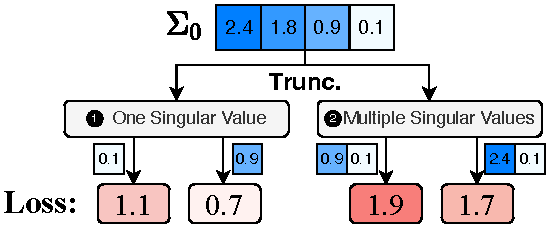
\includegraphics[width=0.45\textwidth]{Figures/white_asvd.pdf}
\label{fig:asvd_whitening}
}
\vline
\hspace{0.1cm}
\centering
\subfigure[Truncation-Aware Data Whitening (\sysname)]{
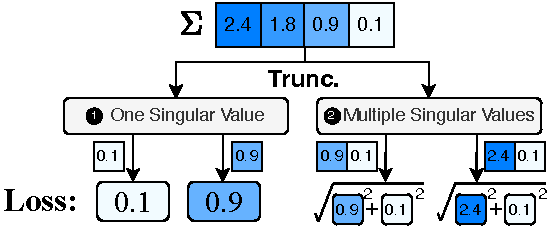
\includegraphics[width=0.45\textwidth]{Figures/white_svdllm.pdf}
\label{fig:svdllm_whitening}
}
\DeclareGraphicsExtensions.
\caption{Compression loss ($L = ||WX-W'X||_F$) of different data preprocessing methods. 
}
\vspace{-2mm}
\label{fig:whitening_comparison}
\end{figure}

\textbf{Key Design:}
The key idea of \sysname is to incorporate a truncation-aware data whitening technique that ensures a \textit{direct} mapping between singular values and compression loss. To achieve this, \sysname enforces the whitened activation $S^{-1}X$ to be orthonormal such that each channel is independent of each other, i.e., $(S^{-1}X)(S^{-1}X)^T= S^{-1}XX^T(S^{-1})^T =I$, where $S$ is derived through Cholesky decomposition~\citep{DBLP:books/siam/Meyer00}. 
%
SVD is then performed on $WS$ to obtain the decomposed matrices $U, \Sigma, V$, where $U=[u_1,u_2,u_3,...,u_r]$, $\Sigma=\text{diag}(\sigma_1,\sigma_2,\sigma_3, \cdots, \sigma_r)$, and $V=[v_1,v_2,v_3,...,v_r]$. Lastly, the smallest singular values in $\Sigma$ are truncated (denoted by $\boldsymbol{\operatorname{Trunc.}}(\Sigma)$) to obtain two low-ranking matrices $W'_u = U\times [\boldsymbol{\operatorname{Trunc.}}(\Sigma)] ^\frac{1}{2}, W'_v = [\boldsymbol{\operatorname{Trunc.}}(\Sigma)] ^\frac{1}{2}\times  V^T \times S^{-1}$ and the compressed weight matrix $W' = W'_u \times W'_v = U \times \boldsymbol{\operatorname{Trunc.}}(\Sigma) \times V^T \times S^{-1}$. 
%
% {\color{red} 
% To save model memory, \sysname replace the original matrix $W$ with the two smaller and low-ranking ones $W_u = U\times [\boldsymbol{\operatorname{Trunc.}}(\Sigma)] ^\frac{1}{2}, W_v = [\boldsymbol{\operatorname{Trunc.}}(\Sigma)] ^\frac{1}{2}\times  V^T \times S^{-1}$ in the compressed LLM.
% }

%%
\cref{fig:svdllm_whitening} illustrates the effect of the proposed truncation-aware data whitening method. In example \ding{182} where only one singular value is truncated, the compression loss equals to the truncated singular value. In example \ding{183}, the compression loss of truncating multiple singular values equals to the square root of the sum of their squares. As such, under the proposed truncation-aware data whitening technique, truncating the smallest singular values leads to minimal compression loss.

%%
In the following, we provide a theoretical proof on why the proposed  truncation-aware data whitening technique ensures a direct mapping between singular values and compression loss in the case of one singular value (\cref{thm:whitening}) and multiple singular values (\cref{col:whitening}), respectively.

\vspace{0mm}
\begin{lemma}
\label{lem:frobenius}
    The Frobenius norm of matrix $A$ with dimension $m\times n$ can be deduced into the square root of the trace of its gram matrix, which is: 
        \begin{equation}
        \|A\|_F \triangleq\left(\sum_{j=1}^n \sum_{i=1}^m\left|a_{i j}\right|^2\right)^{\frac{1}{2}} =\left[\boldsymbol{\operatorname{Trace}}\left(A^T A\right)\right]^{\frac{1}{2}}
        \end{equation}
\end{lemma}
% \vspace{-3mm}
Let $\boldsymbol{\operatorname{SVD}}(WS)$ denote SVD compression on matrix $WS$. The compressed weight matrix $W'$ can be expressed as $W' = \boldsymbol{\operatorname{SVD}}(WS)S^{-1}$. Using \cref{lem:frobenius}, we obtain the compression loss $L_i$ when truncating the $i^{th}$ singular value of $WS$ to reduce its rank for compression:
\begin{equation}
\label{formula:loss}
    \begin{split}
    L_i&=\left\|W X-W^{\prime} X\right\|_F=\left\|W S S^{-1} X-\boldsymbol{\operatorname{SVD}}(W S) S^{-1} X\right\|_F=\left\|(W S-\boldsymbol{\operatorname{SVD}}(W S)) S^{-1} X\right\|_F\\
    &=\left\|\sigma_i u_i v_i^T S^{-1} X\right\|_F=\sigma_i \boldsymbol{\operatorname{Trace}}\left(u_i v_i^T S^{-1} X X^T\left(S^{-1}\right)^T v_i u_i^T\right)^{\frac{1}{2}}
    \end{split}
\end{equation}
Since both $U=[u_1,u_2,u_3,...,u_r]$ and $V=[v_1,v_2,v_3,...,v_r]$ are orthonormal matrices, we have:
\begin{equation}
v_i^T v_i = u_i^T u_i = 1; v_i^T v_j = u_i^T u_j = 0, \forall i \neq j ; \boldsymbol{\operatorname{Trace}}(v_i v_i^T) = \boldsymbol{\operatorname{Trace}}(u_i u_i^T) =1
\end{equation}

\begin{theorem}
\label{thm:whitening}
If $S$ is the Cholesky decomposition of $XX^T$, the compression loss $L_i$ equals to $\sigma_i$.
\end{theorem}
% \vspace{-2mm}
\begin{proof}
\label{proof:whitening}
Since the whitening matrix $S$ is the Cholesky decomposition of $XX^T$, we have $SS^T=XX^T$. We can further infer \cref{formula:loss} to obtain:
\begin{equation}
L_i = \sigma_i \boldsymbol{\operatorname{Trace}}(u_i v_i^T v_i u_i^T)^{\frac{1}{2}} = \sigma_i \boldsymbol{\operatorname{Trace}}\left(u_i\left(v_i^T v_i\right) u_i^T\right)^{\frac{1}{2}}=\sigma_i \boldsymbol{\operatorname{Trace}}\left(u_i u_i^T\right)^{\frac{1}{2}} = \sigma_i \\
\end{equation}
Therefore, $L_i$ of truncating $\sigma_i$ equals to the singular value $\sigma_i$ itself.
\end{proof}
\begin{corollary}
\label{col:whitening}
If $S$ is the Cholesky decomposition of $XX^T$, truncating the smallest singular values leads to the lowest loss $L$ compared to truncating others.
\end{corollary}

% \vspace{-3mm}
\begin{proof}
\label{proof:truncation}
If we truncate $\sigma_{m+1}, \sigma_{m+2}, \sigma_{m+3},..., \sigma_{r}$ in $\Sigma$ for compression, the square of the loss $L$ is:
\begin{equation}
    \begin{split}
    L^2 =& \left|\left| \sum_{i=m+1}^r \sigma_i u_i v_i^T S^{-1}X \right|\right|^2_F =\sum_{j=m+1}^r\sum_{i=m+1}^r\sigma_i\sigma_j\boldsymbol{\operatorname{Trace}}(u_i v_i^T S^{-1}XX^T(S^{-1})^T v_j u_j^T) \\
=& \sum_{i=m+1}^r\sigma_i^2\boldsymbol{\operatorname{Trace}}(u_i v_i^T S^{-1}XX^T(S^{-1})^T v_i u_i^T) = \sum_{i=m+1}^r(L_i )^2=\sum_{i=m+1}^r(\sigma_i)^2
    \end{split}
\end{equation}
The squared loss $L^2$ equals to the sum of the squared singular values (More detailed derivation is in Appendix~\ref{appendix:compression_loss_svdllm}). Truncating the smallest singular values achieves the lowest compression loss.
\end{proof}

%
Given that our proposed truncation-aware data whitening technique is built upon SVD, whose applicability depends on certain singular value distribution, we further conduct a spectrum analysis of the singular values obtained by our technique. We refer the readers to Appendix~\ref{appendix:spectrum_analysis} for details.

%
It should also be noted that our proposed truncation-aware data whitening technique not only ensures a direct mapping between singular values and compression loss, but is also able to achieve the same theoretical optimal compression loss as DRONE~\citep{DBLP:conf/nips/ChenYDH21}.
%
%Apart from aligning the SVD truncation with the compression loss, our data whitening method can even achieve the minimum compression loss, as been done in previous work DRONE~\citep{DBLP:conf/nips/ChenYDH21} on small LMs. 
%
However, during SVD compression, DRONE stores all input activations in memory, which poses a challenge for LLM compression due to high memory consumption.
%However, due to the requirement of caching all input activations, DRONE is difficult to be applied for LLM compression due to significant memory consumption. 
%
In contrast, \sysname incrementally updates its $XX^T$ matrix by adding the $xx^T$ of each new input $x$,  which is considerably smaller than the full input activation.
%
In~\cref{appendix:comparison_with_drone}, we provide our proof on \sysname achieving the same theoretical optimal compression loss as DRONE and discuss the advantages of \sysname over DRONE in memory saving, compression speed, and numerical stability in details.
%Compared with DRONE, SVD-LLM makes improvements in terms of memory, speed, and numerical stability. 
%More detailed analysis about the optimality of \sysname and comparison with DRONE are provided in~\cref{appendix:comparison_with_drone}.


% \vspace{-3mm}
% \subsection{Layer-Wise Closed-Form Update}
% \label{subsec:layer_wise_close_form_update}
% \textbf{Motivation:}
% Given the same calibration data as input, the compressed weight matrix $W'$ generates a new activation $X'$ that is different from $X$ generated by the original weight matrix $W$. As the compression ratio increases, $W$ needs to truncate a larger number of singular values to obtain $W'$, thus $X'$ deviates further from $X$. Therefore, it becomes necessary to design a strategy for updating $W'$ to minimize $||WX'-W'X'|| _F$. However, existing SVD-based LLM compression methods have no design of parameter update after compression, leading to less competitive performance at high compression ratios.

% \begin{wrapfigure}{r}{0.45\textwidth} % "r" 表示右侧，"0.5\textwidth" 控制宽度
%   \centering
%   \vspace{-5mm}
%   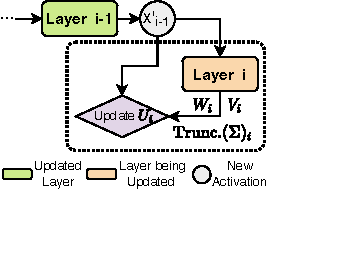
\includegraphics[width=0.31\textwidth]{Figures/updating_strategy_1.pdf} % 调整图像大小
%   \caption{Layer-Wise Closed-Form Update.}
%    \label{fig:local_update}
% \end{wrapfigure}
% \textbf{Key Design:}
% %
% The key idea of \sysname is to incorporate a layer-wise closed-form strategy to update $W'$ to minimize $||WX'-W'X'|| _F$. \cref{fig:local_update} illustrates the overall process. To perform the update in layer $i$, \sysname uses the new activation $X'_{i-1}$ from the previous layer $i-1$ that has been updated. To perform the update without destroying the low-rank structure of $W'_{i}$, \sysname only updates the matrix $U_{i}$ to its closed-form solution $U'_i$ while keeping $\text{Trunc.}(\Sigma)_i$ and $V_i$ fixed as: 
% \begin{equation}
% \label{eq:close_form}
%     \begin{split}
%     % U_i' = \arg \min_{U'} || WX' - W'X'||_F = \arg \min_{U'} || WX' - U'\Sigma_1 V^T S^{-1}X'||_F
%     U_i' &= \arg \min_{U_i} || W_i X'_{i-1} - W'_i X'_{i-1}||_F \\
%     &=  \arg \min_{U_i} || W_i X'_{i-1} - U_i \text{Trunc.}(\Sigma)_i \times V_i^T \times S_i^{-1}X'_{i-1}||_F\\
%     &= W_i X'_{i-1} D^T (D D^T)^{-1}, \text{where } D = \text{Trunc.}(\Sigma)_i V_i^TS_i^{-1} X'_{i-1}
%     \end{split}
% \end{equation}
% \vspace{-3mm}

\subsection{Parameter Update with Sequential Low-rank Approximation}
\label{subsec:lora_finetunig}
\textbf{Motivation:} 
%
Although the proposed truncation-aware data whitening technique helps preserve the accuracy during compression, as the compression ratio increases, the accuracy of the compressed LLM may degrade given that more larger singular values will be truncated by SVD compression.
% Although the truncation-aware data whitening method helps \sysname to reduce the compression loss in each layer of LLMs, this layer-wise compression, which has been commonly applied in many post-training LLM compression works, is difficult to ensure the global minimization of the performance drop of the compressed LLM, especially under the high compression ratio. 
% % As we can see in Figure xxx, when the compression ratio is higher than 0.5, indicating that more than 50\% of the parameter reduction, the perplexity of the compressed LLM drops significantly. 
Therefore, it is necessary to update the remaining parameters in the compressed LLM.


\textbf{Key Design:} 
%
%Driven by previous post-training LLM compression works~\citep{DBLP:conf/nips/MaFW23}, 
\sysname proposes a variant of LoRA fine-tuning to update the remaining weight parameters of the compressed LLM for accuracy recovery. 
%
Specifically, given the two low-ranking matrices $W'_u, W'_v$ generated by truncation-aware data whitening,
%, as discussed in the pseudocode in Appendix~\ref{appendix:pseudocode}. 
%which would break its low-rank structure, 
instead of directly applying LoRA fine-tuning to the compressed weight matrix $W' = W'_u\times W'_v$ as standard LoRA does, we propose to apply LoRA on top of $W'_u$ and $W'_v$ separately to preserve their low-rank structures as follows:
\begin{align}
    W'_u \leftarrow W'_u + B_uA_u, W'_v\leftarrow W'_v + B_vA_v
\end{align}
where $A_u$, $B_u$, $A_v$, and $B_v$ are matrices used for LoRA fine-tuning. 

%
Simultaneously fine-tuning $W'_u$ and $W'_v$ will not guarantee a decrease in fine-tuning loss. This is because the derivatives of $W'_u$ and $W'_v$ are interdependent during the fine-tuning process, where optimization of one matrix may interfere with the optimization of the other. 
%As a result, the overall effect on the fine-tuning loss function may not always lead to a reduction in loss. 
%
Therefore, as shown in Figure~\ref{fig:framework}, we propose a sequential low-rank approximation strategy to fine-tune $W'_u$ and $W'_v$ in a sequential manner. 
%
Specifically, we first freeze matrix $W'_v$ and fine-tune $W'_u$ with LoRA. We then perform the second-round LoRA fine-tuning on matrix $W'_v$ while freezing the updated weight matrix $W'_u$. Finally, we add $B_u\times A_u$ and $B_v\times A_v$ matrices to $W'_u$ and $W'_v$ to obtain the final compressed weight matrices.
